 In this section, we formulate our baseline mathematical model, which
additionally to the transmission dynamics, includes vaccination. In
order to
build our model, we follow the classical Kermack-McKendrick approach.
Figure~\ref{Fig:SchemeModel} shows the compartmental diagram of our
mathematical model.
\begin{figure}[h!]
    \centering
    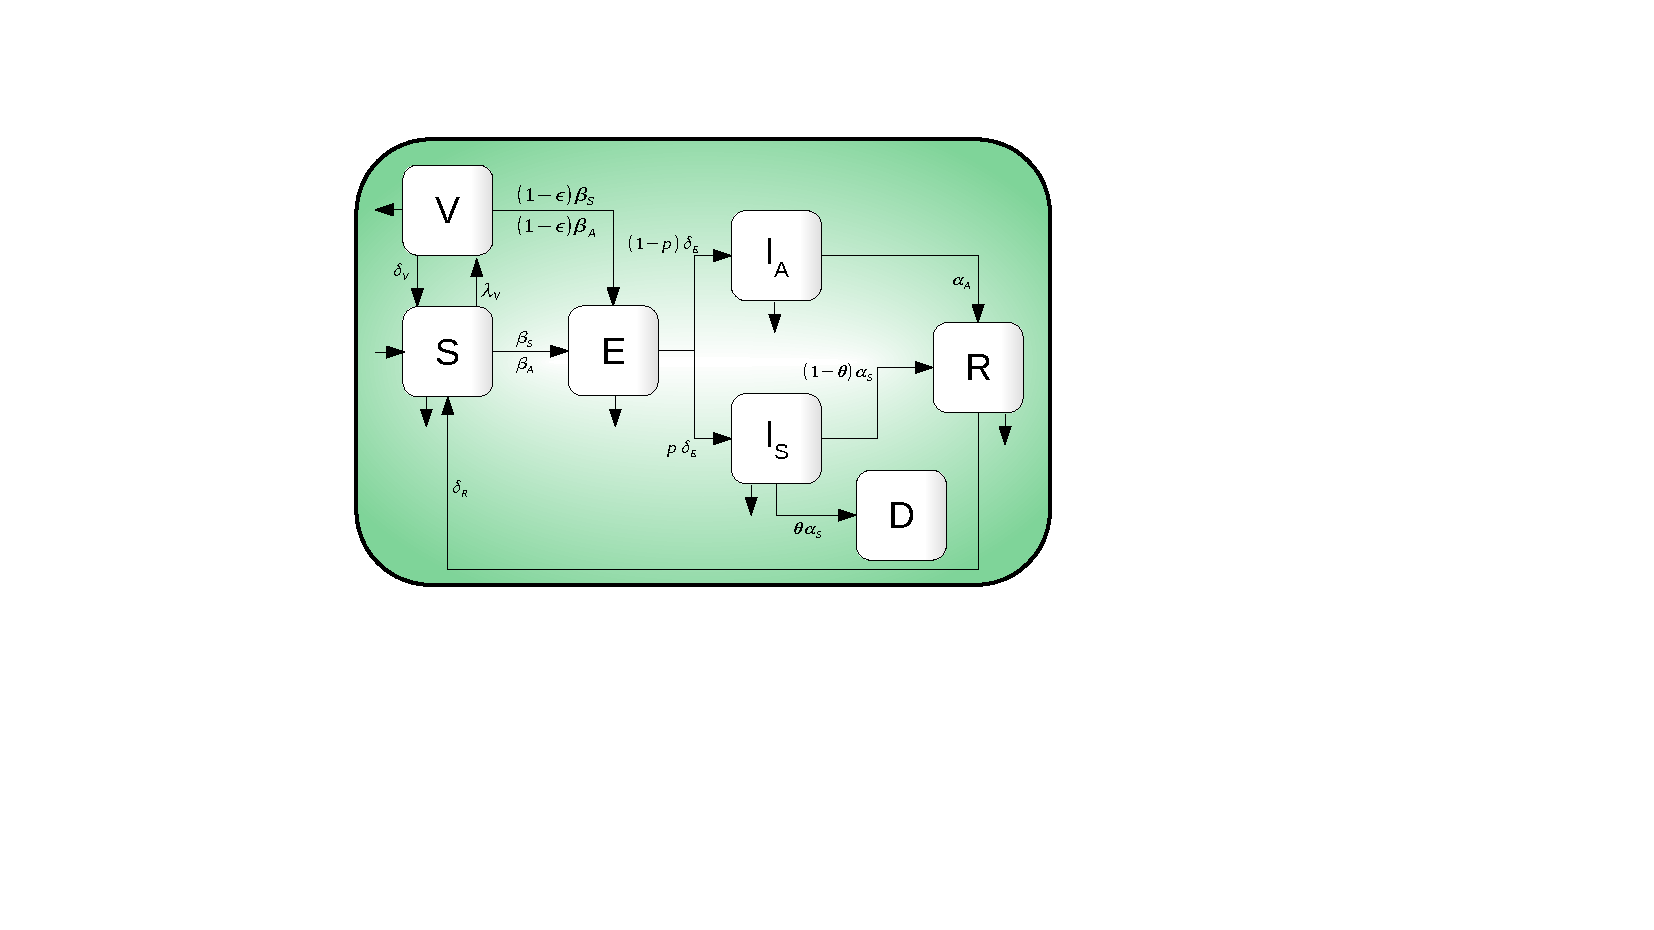
\includegraphics[scale = 1]{SchemeModel_0211_v3.pdf}
    \caption{Compartmental diagram of COVID-19 transmission dynamics
    which
  including vaccination dynamics. Here, there are seven different
  classes:
        Susceptible $(S)$, exposed $(E)$, symptomatic infected
        $(I_S)$,
        asymptomatic infected $(I_A)$, recovered $(R)$, death $(D)$
        and
      vaccinated $(V)$ individuals. It is important to mention that
      $I_{S}$
      represents the proportion of symptomatic individuals who will
      later
      report to some health medical center.}
  \label{Fig:SchemeModel}
\end{figure}

\textcolor{blue}{
    Information about reinfection dynamics on COVID-19 disease
    remains unclear
to date. However, to evaluate scenarios related to this dynamic, we
assume
that reinfection is possible, leading a natural immunity period.
We made the following vaccination modeling hypothesis:
\begin{enumerate}[(H-1)]
    \item
        A vaccine is applied to
        all alive individuals excepting those with symptoms.
        Thus, vaccine doses are applied indiscriminately over
        individuals on
        the $S$, $E$, $I_A$, and $R$ classes;
    \item
        the regarding vaccine is preventive, that is,
        only reflects a favorable response in susceptible
        individuals
        $(S)$;
    \item
        people will only get one vaccine dose during the campaign;
    \item
        the underlying vaccine is imperfect at level
        $(1 -\epsilon) \in(0.5, 9)$, where $\epsilon$ denotes
        vaccine efficacy.
        Thus  the fraction $(1 -\epsilon)$ of  vaccinated
        individuals will not
        develop  artificial immunity and remains susceptible.
\end{enumerate}
Under above hypothesis, our vaccination models is governed by the
following
system pf ordinary differential equations.}
\begin{equation}
    \label{model1}
    \begin{aligned}
        S'(t) &=
            \mu \bar{N} - \frac{\beta_S I_S + \beta_AI_A}{\bar{N}}S
            - (\mu+\lambda_V) S
            + \delta_V V + \delta_R R
        \\
        E'(t)&=
            \frac{\beta_S I_S + \beta_AI_A}{\bar{N}}S
            + (1-\epsilon)
            \frac{\beta_S I_S + \beta_AI_A}{\bar{N}}V-(\mu+\delta_E)
            E \\
        I'_S(t)&=
            p \delta_E E
            -(\mu+\alpha_S) I_S
            \\
        I'_A(t)&=
            (1-p) \delta_E E
            -(\mu + \alpha_A) I_A
        \\
        R'(t)&=
            (1-\theta) \alpha_S I_S
            + \alpha_A I_A
            - (\mu+\delta_R) R
        \\
        D'(t)&=
            \theta \alpha_S I_S
        \\
        V'(t)&=
            \lambda_V S-(1-\epsilon)
            \frac{\beta_S I_S + \beta_A I_A}{\bar{N}}V
            - (\mu+\delta_V) V,
        \end{aligned}
    \end{equation}
where $\bar{N}(t)=S(t)+E(t)+I_S(t)+I_A(t)+R(t)+V(t)$ and
$N=\bar{N}+D$.
We also include the counter equations
\begin{equation}
    \label{eqn:model1_counters}
    \begin{aligned}
        X'(t) &=
            \lambda_V(S + E + I_A + R)
        \\
        Y'_{I_S}(t) &=p
            \delta_E E,
        \\
    \end{aligned}
\end{equation}
where $X(t)$ counts the accumulated applied vaccine doses at
time $t$, and $Y_{I_S}(t)$ count incidence.
Likewise, incidence per day of
infected symptomatic individuals at the $kth$ day can be estimated by
\begin{equation*}
    I_{SA}(k) = Y_{I_S}(k) - Y_{I_S}(k-1)=\int_{k-1}^k p\delta_EE dt.
\end{equation*}
We describe the parameters of system~\eqref{model1} in \Cref{table1}.
%
\begin{table}[h!]
\centering
    \begin{tabular}{cl}
        \toprule
        Parameter & Description
        \\
        \midrule
            $\mu$ &  Death rate
        \\
            $\beta_S$
            & Infection rate between susceptible and symptomatic
            infected
        \\
            $\beta_A$
            &
            Infection rate between susceptible and asymptomatic
            infected
        \\
            $\lambda_V$
            & Vaccination rate
        \\
            $\delta_{V}^{-1}$
            & Immunity average time by vaccination
        \\
            $\epsilon$
            & vaccine Efficacy
        \\
            $\delta_{E}^{-1}$
            &
            Average time of the incubation period
        \\
            $p$
            & \textcolor{red}{Proportion of symptomatic individuals}
        \\
            $\alpha_{S}^{-1}$
            &  Average output time of symptomatic individuals
            due to death or recovery
        \\
            $\theta$
            & Proportion of symptomatic individuals
             who die due to the disease
        \\
            $\alpha_{A}^{-1}$
            & Recovery average time of asymptomatic
            individuals
        \\
            $\delta_{R}^{-1}$
            & Immunity average time by disease
        \\
        \bottomrule
    \end{tabular}
    \caption{Parameters definition of System~\eqref{model1}.}
    \label{table1}
\end{table}
